% !TeX encoding   = UTF-8
\documentclass[msc]{ppgccufmg} % ou [msc] para dissertações
                                        % de mestrado. Para propostas ou
                                        % projetos, usar [phd,project],
                                        % [msc,proposal], etc.
\usepackage[brazil]{babel} % ajusta vários detalhes para
                           % documentos escritos em português,
                           % principalmente hifenização
\usepackage[T1]{fontenc}   % permite a hifenização de
                           % palavras acentuadas
\usepackage[utf8x]{inputenc} % ou [utf8x] para quem prefere
                             % usar a codificação UTF-8
\usepackage{graphicx} % define o comando \includegraphics
                      % para a inclusão de Figuras
%\usepackage[square]{natbib} % permite citações naturalmente
                            % integradas ao texto
\usepackage[a4paper,
portuguese,
bookmarks=true,
bookmarksnumbered=true,
linktocpage,
colorlinks=true,
citecolor=black,
urlcolor=black,
linkcolor=black,
filecolor=black,
]{hyperref}
\usepackage[table,xcdraw]{xcolor}
\usepackage{amsmath}

\usepackage{todonotes}
\usepackage{pdfpages}
\begin{document}

\ppgccufmg{
title={Um Estudo de Ferramentas de \\
Gerenciamento de Requisição de Mudança},
author={Vagner Clementino},
authorrev={Clementino, Vagner},
university={Universidade Federal de Minas Gerais},
course={Ciência da Computação},
address={Belo Horizonte},
date={2016-12},
advisor={Rodolfo F. Resende},
keywords={Manutenção de Software, Ferramentas, Extensões},
%approval={img/approvalsheet.eps},
%approval=[-2.5cm][1]{aprovalsheet},
abstract={Resumo}{resumo},
abstract=[english]{Abstract}{abstract},
abstract={Resumo Estendido}{resumoest},
dedication={dedicatoria},
ack={agradecimentos},
epigraphtext={A verdade é o contrário da mentira, \\
    e a mentira é o oposto da verdade.}{Autor desconhecido},
indexkeys={1.~Computação --- Teses. 2.~Redes --- Teses. I.~Orientador.
    II.~Título.},
}


\chapter{Introdução}
\label{ch:intro}

Dentro do ciclo de vida de um produto de software o processo de manutenção tem
papel fundamental. Devido ao seu alto custo, em alguns casos chegando a 60\%
do custo final \cite{kaur2015review}, as atividades relacionadas a manter e evoluir software tem sua importância considerada tanto pela comunidade científica quanto pela indústria.

A \textit{Manutenção}, dentre outros aspectos, corresponde ao processo de modificar um componente ou sistema de software após a sua entrega com o objetivo de \textit{corrigir falhas, melhorar o desempenho ou adaptá-lo devido à mudanças ambientais} \cite{{159342}}. De maneira relacionada, \textit{Manutenibilidade} é a propriedade de um sistema ou componente de software em relação ao grau de \textit{facilidade} que ele pode ser corrigido, melhorado ou adaptado \cite{{159342}}.

As manutenções em software podem ser divididas em \textit{Corretiva, Adaptativa, Perfectiva e Preventiva} \cite{Lientz:1980:SMM:601062,159342}. A Manutenção Corretiva lida com a reparação de falhas encontradas. A Adaptativa tem o seu foco na adequação do software devido à mudanças ocorridas no ambiente em que ele está inserido. A Perfectiva trabalha para detectar e corrigir falhas latentes antes que elas se manifestem como tal. A  Perfectiva fornece melhorias na documentação, desempenho ou manutenibilidade do sistema. A Preventiva se preocupa com atividades que possibilitem aumento da manutenibilidade do sistema. A \textit{ISO 14764} \cite{1703974} propõe a divisão da tarefa de manutenção nos quatro tipos descritos anteriormente e agrupa-os em um termo único denominado \textit{Requisição de Mudança - Modification Request (RM)}, conforme pode ser visto pela Figura \ref{fig:modification-request}

\begin{figure}[hbtp]
\centering
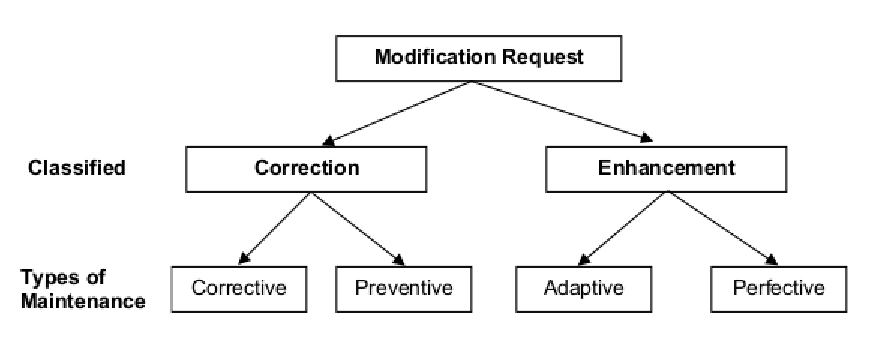
\includegraphics[width=.75\textwidth]{../img/modification_request.eps}
\caption{Tipos de manutenção segundo a norma ISO/IEC 14764. Extraído de
  \cite{1703974}}
\label{fig:modification-request}
\end{figure}


Por conta do volume das Requisições de Mudança se faz necessária a utilização de ferramentas com o objetivo de gerenciá-las. Esse controle é geralmente realizado por Sistemas de Controle de Demandas (SCD)- Issue Tracking Systems, que auxiliam os desenvolvedores na correção de forma individual ou colaborativa de defeitos (bugs), no desenvolvimento de novas funcionalidades, dentre outras tarefas relativas à manutenção de software. Não existe na literatura uma nomenclatura comum para este tipo de ferramenta. Em alguns estudos é possível verificar nomes tais como Sistema de Controle de Defeito - Bug Tracking Systems, Sistema de Gerenciamento da Requisição - Request Management System, Sistemas de Controle de Demandas (SCD)- Issue Tracking Systems e diversos nomes afins. Todavia, de modo geral, o termo se refere as ferramentas utilizadas pelas organizações para \textit{gerir as Requisições de Mudança}. Estas ferramentas podem ainda ser utilizadas por gestores, analistas de qualidade e usuários finais para atividades tais como gerenciamento de projetos, comunicação, discussão e revisões de código. Neste trabalho utilizaremos o termo \texttt{Ferramentas de Gerenciamento de Requisições de Mudança} (FGRM) ao referimos a esta ferramenta. A Tabela \ref{tab:exemplo} apresenta alguns exemplos de ferramentas que podem ser classificadas como FGRM. Também são listados serviços da Internet que oferecem funcionalidades presentes nas FGRM na forma de Software como Serviço.

\begin{table}[ht]
	\centering
	\resizebox{\textwidth}{!}{%
		\begin{tabular}{llll}
			\hline
			\multicolumn{2}{c}{\textbf{Ferramentas}}           & \multicolumn{2}{c}{\textbf{Serviços da Internet}} \\ \hline
			Bugzilla & https://www.bugzilla.org/               & SourceForge    & https://sourceforge.net/    \\ \hline
			MantisBT & https://www.mantisbt.org/               & Lauchpad       & https://launchpad.net/      \\ \hline
			Trac     & https://trac.edgewall.org/              & Code Plex      & https://www.codeplex.com/   \\ \hline
			Redmine  & www.redmine.org/                        & Google Code    & https://code.google.com/    \\ \hline
			Jira     & https://www.atlassian.com/software/jira & GitHub         & https://github.com/         \\ \hline
		\end{tabular}%
	}
	\caption{Exemplos de ferramentas e serviços da Internet. Adaptado de \cite{cavalcanti2014challenges}}
	\label{tab:exemplo}
\end{table}

Grande parte da literatura em manutenção de software trata de técnicas e metodologias tradicionais da Engenharia de Software. Não obstante, é possível verificar um protagonismo das práticas propostas pelos agilistas em projetos de sucesso, mesmo em áreas não relativas à Tecnologia da Informação \cite{Serrador2015}. Neste contexto, verifica-se uma tendência que os departamentos dedicados à manutenção de software se mostrem interessados nas metodologias dos agilistas e que tenham vontade de experimentá-las em suas atividades \cite{Heeager2015}. Apesar da maioria dos textos em Engenharia de Software tratarem desenvolvimento e manutenção como atividades com natureza distintas, esta última pode adaptar características da primeira visando a melhoria do seu desempenho. Dentre as práticas propostas pelos agilistas passíveis de serem utilizadas em tarefas de manutenção é possível citar o desenvolvimento iterativo, maior envolvimento do cliente, comunicação face a face, testes frequentes, dentre outras.

Da mesma forma que ocorre no desenvolvimento de software, é possível verificar uma crescente adoção de técnicas da metodologia ágil na manutenção de software \cite{Soltan2016,Devulapally2015, Heeager2015}. Neste contexto, é natural que ferramentas que dão suporte à manutenção, tal como as FGRM's, tenham que evoluir para se adaptar a esta nova forma de trabalhar. Mesmo em um ambiente tradicional de  desenvolvimento e manutenção de software, verifica-se a necessidade de adequação das FGRM's. Uma das justificativas desta exigência se deve ao fato que a maioria desses sistemas são projetados em torno do termo "demanda" (bug, defeito, bilhete, recurso, etc.), contudo, cada vez mais este modelo parece estar distante das necessidades práticas dos projetos de software \cite{Baysal:2013:SAP:2486788.2486957}.



Apesar da inegável importância das FGRM's, percebe-se um aparente desacoplamento deste tipo de ferramenta com as necessidades das diversas partes interessadas (stakeholders) na manutenção e evolução de software. Um sinal deste distanciamento pode ser observado pelas diversas extensões (plugins) propostas na literatura \cite{101186,Thung:2014:BIT:2635868.2661678,Kononenko:2014:DED:2591062.2591075}. Neste sentido, este trabalho de dissertação se propõe a investigar e contribuir no entendimento de como as Ferramentas de Gerenciamento de Requisição de Mudança estão sendo melhoradas ou estendidas no contexto da transformação do processo de desenvolvimento e manutenção de software de um modelo tradicional para outro que incorpora cada vez mais as práticas propostas pelos agilistas. O intuito é analisar como as FGRM estão sendo modificadas com base na literatura da área em contraste com o ponto de vista dos profissionais envolvidos em manutenção de software.
 
\section{Justificativa}
\label{sec:intro-justificativa}
Desde o final da década de 1970 \cite{Zelkowitz:1979:PSE:578504} percebe-se o aumento do custo referente as atividades de  manutenção de software. Nas décadas de 1980 e 1990 alguns
trabalhos tiveram seu foco no desenvolvimento de modelos de mensuração do custo
para manter o software \cite{Herrin:1985:SMC:323287.323383,hirota1994approach}. Apesar da evolução das metologias de manutenção a estimativa é que nas últimas duas décadas o custo de manutenção tenha aumentado em 50\% \cite{koskinen2010software}. Esta tendência pode ser observada na Figura \ref{fig:software-maintence-costs} no qual é possível verificar a evolução do custo da manutenção de software como fração do custo total do produto.

\begin{figure}
\centering
\includegraphics[width=0.7\linewidth]{../img/software-maintence-costs}
\caption{Evolução da manutenção de software como percentual do custo total.	Extraído de	\cite{engelbertink2010save}}

\label{fig:software-maintence-costs}
\end{figure}

Diante da maior presença de software em todos os setores da sociedade
existe um interesse por parte da academia e da industria no desenvolvimento de
processos, técnicas e \textit{ferramentas} que reduzam o esforço e o custo das tarefas
de desenvolvimento e manutenção de software. Neste linha, o trabalho de Yong \& Mookerjee \cite{1423995}  propõe um modelo que reduz os custos de manutenção e reposição durante a vida útil de um sistema de software. O modelo demonstrou que em algumas situações é \textit{melhor substituir um sistema do que mantê-lo}. Este problema é agravado tendo em vista que o custo de manutenção pode chegar a 60\% do custo total do software \cite{kaur2015review}. Este percentual reflete a fração de desenvolvedores dedicados à tarefas de manutenção de sistemas \cite{Zhang_2003}.

A manutenção não necessariamente exige que o processo de software envolvido
seja o tradicional. Percebe-se alguns exemplos de adoção das práticas ágeis
para fins de manutenção e evolução do software \cite{kajko2009model, Heeager2015, Devulapally2015,Naz2016}. Tal
tendência não é surpreendente tendo em vista que os métodos ``ágeis'' enfatizam
características úteis à eficiência da implementação de software, tais como desenvolvimento incremental e teste contínuo que agregam valor para a evolução e manutenção eficaz de um sistema
\cite{thomas2006agile}. Dentro desta tendência verifica-se a necessidade de que as ferramentas envolvidas no suporte à manutenção de software se adequem à este nova forma de manter software. 

O desenvolvimento e a manutenção de software envolvem diversos tipos de métodos,
técnicas e ferramentas. Em especial no processo de manutenção, um importante aspecto são as diversas Requisições de Mudanças que devem ser gerenciadas. Este controle é realizado pelas Ferramentas de Gerenciamento de Requisição de Mudanças (FGRM) cujo o uso vem crescendo em importância, sobretudo, por sua utilização por gestores, analistas da qualidade e usuários finais para atividades como tomada de decisão e comunicação.

A utilização de  \textit{``demanda''} como conceito central para Ferramentas de Gerenciamento de Requisição de Mudanças (FGRM) parece ser distante das necessidades práticas dos projetos de software, especialmente no ponto de vista dos desenvolvedores \cite{Baysal:2013:SAP:2486788.2486957}. Um exemplo deste desacoplamento das FGRM com a necessidade de seus usuários pode ser visto no trabalho proposto por Baysal \& Holme \cite{baysal2012qualitative} no qual desenvolvedores que utilizam o Bugzilla\footnote{\url{https://www.bugzilla.org}} relatam a
dificuldade em manter uma compreensão global das RM's em que eles estão
envolvidos. Segundo os desenvolvedores seria interessante que a ferramenta
tivesse um suporte melhorado para a Consciência Situacional - Situational
Awareness. Em síntese, eles gostariam de estar cientes da situação global do
projeto bem como das atividades que outras pessoas estão realizando. Um outro
sinal da necessidade de evolução deste tipo de ferramenta pode ser observado considerando as diversas extensões (plugins) propostas na literatura \cite{101186,Thung:2014:BIT:2635868.2661678,Kononenko:2014:DED:2591062.2591075}.

Neste contexto, é proposto neste projeto de dissertação a elaboração de um estudo das Ferramentas de Gerenciamento de Requisição de Mudança (FGRM) como o objetivo de \textit{(i)} entender os requisitos comuns deste tipo de ferramenta; \textit{(ii)} mapear as extensões para as FGRM que estão sendo propostas na literatura; \textit{(iii)} avaliar sobre o ponto de vista dos profissionais a situação atual dos FGRM; \textit{(iv)} propor novas extensões para as FGRM. Vamos discutir os aspectos que são
considerados mais importantes a partir da literatura da área bem como do ponto de vista de profissionais envolvidos em manutenção de software. De forma particular, iremos estudar os mecanismos de personalização que algumas destas ferramentas permitem e tentaremos ainda criar exemplos de personalização para alguma possível extensão a ser identificada ao longo do trabalho.

\section{Motivação}
\label{sec:intro-motivacao}

\section{Problema}
\label{sec:intro-problema}

\section{Visão Geral da Proposta}
\label{sec:intro-visao-geral}

\section{Metodologia de Pesquisa}
\label{sec:intro-metodologia}

O trabalho de dissertação pode ser dividido nas etapas listadas a seguir:

\begin{itemize}[(i)]
	\item Mapeamento Sistemático da Literatura \cite{keele2007guidelines}
	\item Caracterização das Ferramentas de Gerenciamento de Requisição de Mudança (FGRM)
	\item Pesquisa (Survey) com os desenvolvedores \cite{wohlin2012experimentation}
	\item Desenvolvimento de extensões para as FGRM's
\end{itemize}

\section{Contribuições da Dissertação}
\label{sec:intro-contribuicao}

\section{Organização da Dissertação}
\label{sec:intro-organizacao-dissertacao}








\chapter{Manutenção de Software: Uma Visão Geral}
\label{ch:visao-geral-manutencao}

Uma tendência natural do software é evoluir a fim de atender aos novos requisitos e alterações no ambiente no qual ele está inserido. Em uma série de estudos Lehman propõe um conjunto de leis sobre a evolução do software. Dentre elas podemos destacar as leis da Mudança Contínua (Continuing
Change) e da Complexidade Crescente (Increasing complexity). Segundo a lei da
Mudança Contínua um programa que é utilizado em um ambiente real deve mudar ou se tornará progressivamente menos útil \cite{lehman1980understanding}. A lei da
Complexidade Crescente (Increasing complexity) afirma que quando um sistema em
evolução muda, sua estrutura tende a se tornar mais complexa. Nesta situação,
recursos extras devem ser disponibilizados a fim de preservar e simplificar a
estrutura do software \cite{lehman1980understanding}. As leis de Lehman tem
sido validadas, especialmente aquelas relacionadas a tamanho e
complexidade do software. Em um trabalho recente Yu \& Mishra \cite{{yu2013empirical}} examinaram de forma empírica as Leis de Lehman em relação a evolução da qualidade do software. Os
resultados dão suporte as Leis especialmente a que versa sobre a qualidade, na qual um produto de software decresce a sua aquele atributo ao longo do tempo, exceto que ele seja reestruturado.

Percebida a importância do processo de manutenção de software, alguns trabalhos foram propostos visando mensurar o seu custo bem como propor processos com o objetivo de reduzir o esforço envolvido neste tipo de atividade.

No trabalho de Herrin \cite{Herrin:1985:SMC:323287.323383} foi proposto um modelo matemático com o
objetivo de avaliar o impacto financeiro no orçamento de uma universidade devido às atividades de manutenção no sistema de processamento de dados da instituição. O modelo propõe que o valor disponível para desenvolvimento de um novo sistema é função inversa do custo de manutenção do software existente. Desta forma, o fato de se manter um sistema durante muito tempo poderá impossibilitar a aquisição ou mesmo o desenvolvimento de um novo.

No estudo de Hirota et al. \cite{hirota1994approach} é proposta a utilização da técnica Análise de Ripple para estimar o custo da manutenção de software. O termo ``efeito Ripple'' foi utilizado pela primeira vez em um artigo publicado por Haney \cite{haney1972module} para descrever a forma que a mudança em um módulo poderia causar alterações em outras partes do sistema \cite{bilal2005using}. A Análise Ripple é, portanto, uma técnica para analisar o fluxo de dados de variáveis dentro de um determinado programa. Os valores retornados pela aplicação do método são denominados Complexidade de Ripple. Os resultados demostraram que a Complexidade de Ripple está mais relacionada ao entendimento do
software do que as métricas padrão, como linhas de código, complexidade ciclomática e pontos de função. Desta forma, a Complexidade de Ripple poderia ser utilizada, por exemplo, para predizer os custo de manutenção de um sistema, bem como a necessidade de substituição do mesmo.

Mediante o uso de Redes Neurais Shula \& Misra
\cite{Shukla:2008:ESM:1342211.1342232} propõe um estudo para medir o custo de
manutenção de software. O trabalho discute a utilização de outras métricas além
de linha de código e pontos de função para medir  tamanho e custo do processo de manutenção. Os resultados demonstraram a possibilidade de construir um modelo para medir o custo utilizando Redes Neurais. Contudo, os resultados são sensíveis a escolha da arquitetura e parâmetros de treino, os quais idealmente deveriam ser preparados por um especialista no sistema (oráculo).


A dinamicidade do ambiente de negócios tem levado a diversas organizações a adotar as metodologias propostas pelos agilistas pelo fato delas auxiliarem no atendimento das exigências do cliente \cite{Devulapally2015}. Esta tendência é mais forte no desenvolvimento de software e nos últimos anos vem ocorrendo de forma gradativa na manutenção. 

No trabalho de Kajko-Mattsson \& Nyfjord \cite{4755767} foi proposto um modelo ágil para manutenção que apropria diferentes práticas do Extreme Programming e do Scrum. Segundo os autores a junção desta duas metodologias possibilita a inclusão de práticas úteis tanto do ponto de vista do gerente do projeto bem como dos desenvolvedores. O modelo encoraja diversas práticas tais como \textit{product backlog}, testes antes da codificação, planejamento iterativo, dentre outras.

A adoção na manutenção de software de algumas práticas propostas pelos agilistas foram analisadas durante 08 meses em estudo realizado por Svensson \& Host \cite{1402140}. Ao utilizar o Extreme Programming (XP) no processo de manutenção os autores concluíram que é muito difícil fazer uso do XP sem que sejam realizadas adequações no desenho de diversas práticas para desta forma adequar às necessidades do time de desenvolvimento.

O estudo Heeager \& Rose \cite{Heeager2015} propõe um conjunto de nove heurísticas com o objetivo de ajudar aos profissionais da manutenção de software na adoção de práticas propostas pelos agilistas. O trabalho consistiu da inclusão do Scrum na rotina de trabalho do departamento de manutenção de software de uma organização de grande porte. Os autores argumentam que os métodos ágeis, quando aplicado ao trabalho de desenvolvimento, têm certas características relativamente bem compreendidas, no entanto o trabalho de manutenção difere do de desenvolvimento em certos aspectos e, portanto, é desafiador a implementação de métodos ágeis em um departamento de manutenção.

Diante da crescente importância das Ferramenta de Gerenciamento de Requisição de Mudanças (FGRM) no processo de manutenção de software, diversos trabalhos vêm sendo propostos com o objetivo de entender como elas estão sendo utilizadas bem como sugerir melhorias no desenho para desenvolver futuras FGRM's.

No trabalho de Junio et al. \cite{5741246} é proposto um processo denominado PASM (Process for Arranging
Software Maintenance Requests) que propõe lidar com tarefas de manutenção como projetos de software. Para tanto, utilizou-se técnicas de análise de agrupamento (clustering) a fim de melhor compreender e comparar as demandas de manutenção. Os resultados demostraram que depois de adotar o PASM os
desenvolvedores tem dedicado um tempo maior para análise e validação. De outra forma, relacionada um menor tempo foi dedicado às tarefas de execução e codificação.

No estudo realizado por Bettenburg et al. \cite{bettenburg2008makes} foi
desenvolvida uma pesquisa (\textit{survey}) entre desenvolvedores e usuários dos
projetos Apache\footnote{\url{http://www.apache.org/}}, Eclipse\footnote{\url{https://www.eclipse.org}} e Mozilla\footnote{\url{https://www.mozilla.org}} a fim de verificar o que
produziria uma boa FGRM. Os resultados demonstraram que do ponto de vista dos desenvolvedores eram consideradas úteis funcionalidades tais como reprodução do erro, rastros de pilhas (stack traces) e casos de testes. A partir deste resultado foi construído um protótipo capaz de conduzir os usuários na coleta e fornecimento de um maior número de informações úteis para a resolução do defeito reportado.

Avaliando o controle de demandas como um processo social, Bertram et
al. \cite{Bertram:2010:CCB:1718918.1718972} realizaram um estudo qualitativo em
FGRM's quando utilizados por pequenas equipes de desenvolvimento de software. Os resultados mostraram que este tipo ferramenta não é apenas um banco de dados de rastreamento de defeitos, recursos ou pedidos de informação, mas também atua como um ponto focal para a comunicação e coordenação para diversas partes interessadas (stakeholders) dentro e fora da equipe de software. Os
clientes, gerentes de projeto, o pessoal envolvido com a garantia da qualidade
e programadores, contribuem em conjunto para o conhecimento compartilhado dentro do contexto das FGRM's.

Em Zimmermann et al. \cite{5070993} é discutido a importância de que a informação descrita em uma Requisição de Mudança seja relevante e completa a fim de que o defeito reportado seja resolvido rapidamente. Contudo, na prática, a informação apenas chega ao desenvolvedor com a qualidade requerida após diversas interações com o usuário afetado. Com o objetivo de minimizar este
problema os autores propõe um conjunto de diretrizes para a construção de um ferramenta capaz de reunir informações relevantes a partir do usuário e identificar arquivos que precisam ser corrigidos para resolver o defeito.

No trabalho de Breu et al.\cite{Breu:2010:INB:1718918.1718973} o foco é analisar o papel dos FGRM's no suporte à colaboração entre desenvolvedores e usuários de um software. A partir da análise quantitativa e qualitativa de uma amostra de defeitos registrados em uma FGRM de dois projetos de software livre, foi possível verificar que os usuários desempenham um papel além de simplesmente reportar uma falha: a participação ativa e permanente dos usuários finais foi importante no progresso da resolução das falhas que eles descreveram.

O desenvolvimento de novas funcionalidades em FGRM's, mediante a capacidade de
extensão propiciada por algumas delas vêm sendo explorada na literatura. \textit{Buglocalizer} \cite{Thung:2014:BIT:2635868.2661678} é uma extensão para o Bugzilla que possibilita a localização dos arquivos do código fonte que estão relacionados ao defeito relatado. A ferramenta extrai texto dos campos de sumário e descrição de um determinado erro reportado no Bugzilla. Este texto é comparado com o código fonte por meio de técnicas de Recuperação da Informação.

\textit{NextBug} \cite{101186} é uma extensão para o Bugzilla que
recomenda novos bugs para um desenvolvedor baseado no defeito que ele esteja
tratando atualmente. O objetivo da extensão é sugerir defeitos com base em técnicas de
Recuperação de Informação.

No trabalho de Kononenko et al. \cite{Kononenko:2014:DED:2591062.2591075} é
apresentada uma ferramenta denominada \textit{DASH} cujo objetivo é agrupar as
demandas que são relevantes para as atividades de um desenvolvedor. Naturalmente todas as demandas ditas relevantes deveriam estar sob a responsabilidade de um mesmo programador. O principal objetivo desta ferramenta é aumentar a Consciência Situacional (Situational Awareness) dos
desenvolvedores. Segundo os autores, o principal ganho do uso da ferramenta é
que os programadores podem gerenciar melhor o excesso de informação e ficar
mais ciente da evolução das demais demandas do sistema.

Na ferramenta proposta por Thung et al. \cite{Thung:2014:DIT:2642937.2648627} o
foco é na determinação de defeitos duplicados. A contribuição deste trabalho é a
integração do estado da arte de técnicas não supervisionadas para detecção de
falhas duplicadas conforme proposto por Runeson et al. \cite{Runeson:2007:DDD:1248820.1248882}. A ferramenta utiliza o Modelo de Vetor Espacial (Vetor Space Model) como métrica de similaridade entre os defeitos e fornece aos desenvolvedores uma lista de possíveis duplicatas.

\chapter{Mapeamento Sistemático da Literatura}
\label{ch:mapeamento-sistematico}





\section{Introdução}
\label{sec:map-intro}
\todo[inline]{OBJETIVO DA SEÇÃO: Esta seção visa apresenta uma visão geral do Mapeamento Sistemáticao realizados. Apresenta, de maneira sucinta, o contexto, o problema, a solução e os resultado deste estudo, de forma resumida, mas abrangente. Idealmente deverá ser a última seção a ser escrita neste Capítulo.}

\section{Metodologia de Pesquisa}
\label{sec:map-metodologia}

Um \textit{Mapeamento Sistemático da Literatura}, também conhecido como Estudos de Escopo (Scoping Studies), tem como objetivo fornecer uma visão geral de determinada área de pesquisa, estabelecer se existem evidências de estudos sobre determinado tema e fornecer uma indicação da quantidade de trabalho na linha de pesquisa sob análise \cite{keele2007guidelines,wohlin2012experimentation}. Nesta dissertação empregamos as diretrizes propostas por \cite{Petersen2008}, de forma a produzirmos uma revisão mais sistemática e forma de modo a propiciar maior facilidade de replicação e extensão deste trabalho. Em particular, foi definido um conjunto de questões de pesquisa que foram utilizadas no processo de busca e seleção dos estudos primários. Em seguida, foram construídos esquemas de classificação com base nos dados extraídos  dos artigos. Por fim, foi realizada a análise e sintetização dos dados. A estrutura desta seção está de acordo com o processo de trabalho executado, de modo que cada subseção representa uma etapa executada.

\subsection{Questões de Pesquisa}
\label{subsec:map-questoes-de-pesquisa}

\begin{itemize}
	\item \textbf{$RQ_1$}: Quais são as funcionalidades propostas para estender as FGRM?
	\item \textbf{$RQ_2$}: Qual técnica foi utilizada para desenvolver a extensão?
	\item \textbf{$RQ_3$}: Quais as FGRM estão sendo estendidas?
	\item \textbf{$RQ_4$}: Como foi realizado o processo de avaliação da extensão proposta?
\end{itemize}

\subsection{Pesquisa da Literatura}
\label{subsec:map-pesquisa-literatura}

\subsection{Esquemas de Classificação}
\label{subsec:map-esquemas-classificacao}


\section{Resultados}
\label{sec:resutaldos}

\section{Limitações e Ameaças à Validade}

\section{Trabalhos Relacionados}

\section{Resumo do Capítulo}

\chapter{Caracterização das Ferramentas de Gerenciamento de Requisição de Mudança}
\label{ch:caracterizacao}


\section{Introdução}

Esta etapa do trabalho consistirá de um estudo exploratório com o objetivo de determinar quais são as funcionalidades comuns às Ferramentas de Gerenciamento de Requisição de Mudança (FGRM). O estudo consistirá na leitura da documentação de alguns FGRM para que de forma sistemática seja levantado quais são as funcionalidades oferecidas pela ferramenta em análise. O método de escolha das FGRM será avaliado posteriormente, todavia, um possível ponto de partida é a lista disponível na Wikipédia que compara diversas FGRM\footnote{\url{https://en.wikipedia.org/wiki/Comparison_of_issue-tracking_systems}}.

O resultado deste estudo permitirá compreender melhor este tipo de ferramenta tomando como base as suas funcionalidades em comum. Também será possível propor extensões para as FGRM (Seção ref{ch:extensoes}) tendo em vista a possibilidade de determinar o conjunto mínimo de funções deste tipo de sistema. Uma outra possível contribuição é desenvolver uma taxonomia deste tipo de ferramenta com base nas funcionalidades oferecidas.

\section{Discussão}

\section{Ameças à Validade}

\section{Replicação da Pesquisa com Profissionais}

\section{Resumo do Capítulo}


\chapter{Pesquisa com Profissionais}
\label{ch:pesquisa-profissionais}

\section{Introdução}
Com o objetivo de coletar os aspectos mais importantes das FGRM's do ponto de
vista dos profissionais ligados à manutenção de software será realizada uma
 pesquisa (survey). O planejamento e o desenho da pesquisa seguirá as diretrizes propostas em \cite{wohlin2012experimentation}.

A população da pesquisa proposta é a comunidade envolvida com o processo de
manutenção de software e que faça uso de FGRM's. Neste contexto, seriam
possíveis amostras, os desenvolvedores envolvidos com tarefas de manutenção nos
projetos da Mozilla\footnote{\url{https://bugzilla.mozilla.org/}} ou da
Eclipse Foundation\footnote{\url{https://bugs.eclipse.org/bugs/}}. Durante a
execução da dissertação será avaliado qual amostra caracteriza melhor a
população do estudo.

\section{Objetivo da Pesquisa}

\section{Metodologia}


\subsection{Questionário}

\subsection{População,Amostra e Respostas}

\section{Análise dos Dados}

\section{Discussão}

\section{Ameças à Validade}

\section{Replicação da Pesquisa com Profissionais}

\section{Resumo do Capítulo}

\chapter{Extensões para Ferramentas de Gerenciamento de Requisição de Mudança}
\label{ch:extensoes}

\section{Introdução}
A partir dos resultados do Mapeamento Sistemática, do Estudo de Caracterização das ferramentas e da Pesquisa com o profissionais pretende-se desenvolver uma ou mais extensão (plugins) para determinada FGRM. Cabe ressaltar que esta parte do trabalho será realizada caso o esforço seja compatível com os prazos e recursos disponíveis. No caso da implementação de um plugin este será apresentado e avaliado mediante a realização de um \textit{Experimento Controlado} \cite{wohlin2012experimentation} utilizando a base de dados de demandas de manutenção de uma empresa de software real. Este experimento será conduzido com o objetivo de avaliar a utilização de uma extensão em um ambiente de desenvolvimento e manutenção de software real.

\section{Ameaças à Validade}

\section{Resumo do Capítulo}

\chapter{Avaliação das Extensões para Ferramentas de Gerenciamento de Requisição de Mudança}

\section{Introdução}

\section{Resumo do Capítulo}

\chapter{Conclusão}
\label{ch:conclusao_trab_futuros}

A Manutenção de Software é um processo complexo e caro e, portanto,  merece atenção da
comunidade acadêmica e da indústria. Desta forma, emerge a necessidade do desenvolvimento de técnicas, processo e ferramentas que reduzam o custo e o esforço envolvidos nas atividades de manutenção e evolução de software. Neste contexto, as Ferramentas de Gerenciamento de Requisição de Mudança desempenham um papel fundamental que ultrapassa a simples função de registrar falhas em software. Neste sentido é proposto o estudo para entender o papel desta ferramenta, analisar a literatura sobre o assunto e discutir os aspectos que são considerados mais importantes do ponto de vista dos profissionais. Para alcançarmos este objetivo é proposto um Cronograma de Atividade conforme exibido no Anexo \ref{anexo:cronograma}. As atividades que compõe cada etapa do trabalho estão descritas no Anexo \ref{anexo:atividades}.

\chapter*{Apêndices}
\label{ch:apendice}
\appendix
\section{Anexo A}
\label{anexo:cronograma}
\includepdf{../img/Cronograma-Atividades-Dissertacao.pdf}

\section{Anexo B}
\label{anexo:atividades}
\includepdf{../img/Detalhamento-Atividades-Dissertacao.pdf}

% Incluindo bibliografia:
\ppgccbibliography{../bib/bibliografia}
\end{document}
